 13. Put a uniform meter scale horizontally on your extended index fingers with the left one at 0.00 cm and the right one at 90.00 cm. When you attempt to move both the fingers slowly towards the center, initially only the left finger slips with respect to the scale and the right finger does not. After some distance, the left finger stops and the right one starts slipping. Then the right finger stops at a distance \(x_R\) from the center (50.00 cm) of the scale and the left one starts slipping again. This happens because of the difference in the frictional forces on the two fingers. If the coefficients of static and dynamic friction between the fingers and the scale are 0.40 and 0.32, respectively, the value of \(x_R\) (in cm) is \(\boxed{~\hspace{1.0cm}~}\).

\begin{center}
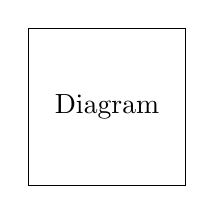
\begin{tikzpicture}
  \node [draw, minimum width=2cm, minimum height=2cm] {Diagram};
\end{tikzpicture}
\end{center}